\documentclass[hidelinks]{article}
\usepackage[letterpaper,margin=1.0in]{geometry}
\usepackage[utf8]{inputenc}
\pagenumbering{arabic}
\usepackage{authblk}
\usepackage{graphicx}
\usepackage[singlelinecheck=false]{caption} % singlelinecheck makes single line caption left aligned instead of centered
\usepackage{subcaption}
\usepackage{amsmath}
\usepackage[round]{natbib}
\usepackage{fancyhdr}
\usepackage{longtable}
\usepackage{booktabs}
% hyperlinks
\usepackage{hyperref}

\usepackage{xspace}
\usepackage{mathrsfs}
\usepackage{graphicx}

\pagestyle{fancy}
\fancyhead[R]{\textbf{Expanding \stdpopsim}}

% for highlighting text
\usepackage{xcolor}
\usepackage{soul}

% bibliography
\usepackage[round]{natbib}   % omit 'round' option if you prefer square brackets
\bibliographystyle{plainnat}



\newcommand{\Stdpopsim}{\texttt{Stdpopsim}\xspace}
\newcommand{\stdpopsim}{\texttt{stdpopsim}\xspace}

%commands to format figure and table references in the supplement
\newcommand{\beginsupplement}{%
        \fancyhead[L]{Supplemental Material}
        \setcounter{table}{0}
        \renewcommand{\thetable}{S\arabic{table}}%
        \setcounter{figure}{0}
        \renewcommand{\thefigure}{S\arabic{figure}}%
     }
\newcommand{\stopsupplement}{%
        \setcounter{table}{0}
        \renewcommand{\thetable}{\arabic{table}}%
        \setcounter{figure}{0}
        \renewcommand{\thefigure}{\arabic{figure}}%
     }

\makeatletter
\newcommand{\labelname}[1]{\def\@currentlabelname{#1}}
\makeatother

% Avoid pandoc bug when there are lists in the body.
\providecommand{\tightlist}{%
\setlength{\itemsep}{0pt}\setlength{\parskip}{0pt}}

\title{Adding selection to \stdpopsim: oh how the tables have turned}


% \author[1,+]{M. Elise Lauterbur}
% \author[2,*]{Maria Izabel A. Cavassim}
% \author[3,*]{Ariella L. Gladstein}
 \author[4,*]{Graham Gower}
 \author[5*]{Nathaniel S. Pope}
% \author[6,*]{Georgia Tsambos}
% \author[5,7]{Jeff Adrion}
% \author[5]{Saurabh Belsare}
% \author[8]{Arjun Biddanda}
% \author[5]{Victoria Caudill}
% \author[9]{Jean Cury}
% \author[10]{Ignacio Echevarria}
% \author[11]{Benjamin C. Haller}
% \author[12,13]{Ahmed R. Hasan}
% \author[14,15]{Xin Huang}
% \author[16]{Leonardo Nicola Martin Iasi}
% \author[17]{Ekaterina Noskova}
% \author[18]{Jana Obšteter}
% \author[19]{Vitor Antonio Corrêa Pavinato}
% \author[20,21]{Alice Pearson}
% \author[22,23]{David Peede}
% \author[24]{Manolo F. Perez}
% \author[5]{Murillo F. Rodrigues}
% \author[5]{Chris C. R. Smith}
% \author[25]{Jeffrey P. Spence}
% \author[5]{Anastasia Teterina}
% \author[5]{Silas Tittes}
% \author[26]{Per Unneberg}
% \author[27]{Juan Manuel Vazquez}
% \author[28]{Ryan K. Waples}
% \author[29]{Anthony Wilder Wohns}
% \author[30]{Yan Wong}
% \author[31]{Franz Baumdicker}
% \author[32]{Reed A. Cartwright}
% \author[33]{Gregor Gorjanc}
% \author[34]{Ryan N. Gutenkunst}
% \author[30]{Jerome Kelleher}
% \author[5]{Andrew D. Kern}
% \author[35]{Aaron P. Ragsdale}
% \author[5,36]{Peter L. Ralph}
% \author[37]{Daniel R. Schrider}
% \author[38,+]{Ilan Gronau}


 \affil[*]{\small{These authors contributed equally to the paper.}}
% \affil[+]{\small{Corresponding authors: lauterbur@gmail.com ; ilan.gronau@runi.ac.il.}}
% \affil[1]{\small{Department of Ecology and Evolutionary Biology, University of Arizona, Tucson AZ 85719, USA}}
% \affil[2]{\small{Department of Ecology and Evolutionary Biology, University of California, Los Angeles, Los Angeles CA, USA}}
% \affil[3]{\small{Embark Veterinary, Inc., Boston MA 02111, USA}}
 \affil[4]{\small{Section for Molecular Ecology and Evolution, Globe Institute, University of Copenhagen, Denmark}}
 \affil[5]{\small{Institute of Ecology and Evolution, University of Oregon, Eugene OR 97402, USA}}
% \affil[6]{\small{School of Mathematics and Statistics, University of Melbourne, Australia}}
% \affil[7]{\small{AncestryDNA, San Francisco CA 94107, USA}}
% \affil[8]{\small{54Gene, Inc., Washington DC 20005, USA}}
% \affil[9]{\small{Université Paris-Saclay, CNRS, INRIA, Laboratoire Interdisciplinaire des Sciences du Numérique, UMR 9015 Orsay, France}}
% \affil[10]{\small{School of Life Sciences, University of Glasgow, Glasgow, UK}}
% \affil[11]{\small{Department of Computational Biology, Cornell University, Ithaca NY, USA}}
% \affil[12]{\small{Department of Cell and Systems Biology, University of Toronto, Toronto ON, Canada}}
% \affil[13]{\small{Department of Biology, University of Toronto Mississauga, Mississauga ON, Canada}}
% \affil[14]{\small{Department of Evolutionary Anthropology, University of Vienna, Vienna, Austria}}
% \affil[15]{\small{Human Evolution and Archaeological Sciences (HEAS), University of Vienna, Vienna, Austria}}
% \affil[16]{\small{Department of Evolutionary Genetics, Max Planck Institute for Evolutionary Anthropology, Leipzig, Germany}}
% \affil[17]{\small{Computer Technologies Laboratory, ITMO University, St Petersburg, Russia}}
% \affil[18]{\small{Agricultural Institute of Slovenia, Department of Animal Science, Ljubljana, Slovenia}}
% \affil[19]{\small{Entomology Department, The Ohio State University, Wooster OH, USA}}
% \affil[20]{\small{Department of Genetics, University of Cambridge, Cambridge, UK}}
% \affil[21]{\small{Department of Zoology, University of Cambridge, Cambridge, UK}}
% \affil[22]{\small{Department of Ecology, Evolution, and Organismal Biology, Brown University, Providence RI, USA}}
% \affil[23]{\small{Center for Computational Molecular Biology, Brown University, Providence RI, USA}}
% \affil[24]{\small{Department of Genetics and Evolution, Federal University of Sao Carlos, Sao Carlos 13565905, Brazil}}
% \affil[25]{\small{Department of Genetics, Stanford University School of Medicine, Stanford CA 94305, USA}}
% \affil[26]{\small{Department of Cell and Molecular Biology, National Bioinformatics Infrastructure Sweden, Science for Life Laboratory, Uppsala University, Husargatan 3, SE-752 37 Uppsala, Sweden}}
% \affil[27]{\small{Department of Integrative Biology, University of California, Berkeley, Berkeley CA, USA}}
% \affil[28]{\small{Department of Biostatistics, University of Washington, Seattle WA, USA}}
% \affil[29]{\small{Broad Institute of MIT and Harvard, Cambridge MA 02142, USA}}
% \affil[30]{\small{Big Data Institute, Li Ka Shing Centre for Health Information and Discovery, University of Oxford, Oxford OX3 7LF, UK}}
% \affil[31]{\small{Cluster of Excellence - Controlling Microbes to Fight Infections, Eberhard Karls Universität Tübingen, Tübingen, Baden-Württemberg, Germany}}
% \affil[32]{\small{School of Life Sciences and The Biodesign Institute, Arizona State University, Tempe AZ, USA}}
% \affil[33]{\small{The Roslin Institute and Royal (Dick) School of Veterinary Studies, University of Edinburgh, Edinburgh EH25 9RG, UK}}
% \affil[34]{\small{Department of Molecular and Cellular Biology, University of Arizona, Tucson AZ 85721, USA}}
% \affil[35]{\small{Department of Integrative Biology, University of Wisconsin-Madison, Madison WI, USA}}
% \affil[36]{\small{Department of Mathematics, University of Oregon, Eugene OR 97402, USA}}
% \affil[37]{\small{Department of Genetics, University of North Carolina at Chapel Hill, Chapel Hill NC 27599, USA}}
% \affil[38]{\small{Efi Arazi School of Computer Science, Reichman University, Herzliya, Israel}}

\date{\small{\today{}}}

\begin{document}

\maketitle


\section*{Abstract}

\section*{Introduction}
    \label{introduction}
    % natural selection
    Natural selection is a fundamental force in evolution, shaping the
    genetic diversity of populations and driving the adaptation of
    species to their environments. The effects of natural selection
    on genetic variation are complex, and can be difficult to disentangle
    from other evolutionary processes such as mutation, recombination,
    and genetic drift \cite[e.g.,][]{gillespie1991causes}.
    For instance changes in population size can lead to fluctuations
    in genetic diversity across a recombining chromosome 
    that can mimic the effects of selection \citep{simonsen1995properties, barton1998effect},
    and lead to spurious inferences about the strength and targets of genetic adaptation
    \cite{simonsen1995properties,akey2004population,nielsen2005genomic}.
    In turn selection can confound our ability to infer demographic 
    history from allele frequencies \citep{ewing2016consequences} and
    estimates of inverse coalescent rate \citep{schrider2016effects}.
    Thus it is imperative to joingly account for the effects of selection
    and demography when inferring evolutionary history from genetic data
    however this is a challenging task from a modeling perspective.

    % simulation
    To meet this need the field of population genetics
    has turned to simulation.
    Simulation has become a critical tool for interpretation, 
    analysis, and exploration of realistic evolutionary models.
    Simulation in population genetics has a long history 
    including both backward in time coalescent simulations
    \citep{kingman1982genealogy,hudson1983testing, hudson1990gene}
    and forward in time simulations of complex demography and selection
    \citep[e.g.,][]{gillespie1984molecular,thornton2014c++, haller2019slim}.
    The development of simulation tools has been driven by the need to
    understand the effects of complex evolutionary processes on genetic
    variation \citep[e.g.,][]{galloway2020few}, to provide a null model for hypothesis testing
    \citep[e.g.,][]{hudson1992statistical}, to
    to explore the power and limitations of statistical methods \cite[e.g.,]{przeworski2002signature},
    and increasingly to provide a basis for machine learning and other
    simulation-based inference methods \citep[e.g.,]{kern2018diplos}.
    While this is so, joint simulation of complex demography and selection
    is challenging, and requires a deep understanding of the underlying
    evolutionary processes, as well as a number of parameter choices including
    the strength of selection, the distribution of fitness effects, and the
    recombination rate, as well as a parameterized model of demography.
    This is dounting task for many researchers, and can be a barrier to
    the adoption of simulation-based methods in population genetics.
    Further, sharing and comparing simulation results among studies can 
    itself be challenging, as different simulation tools may use different
    models and parameterizations, and may not be directly comparable.
    This is a major limitation for the field, as it can make it difficult
    to assess the robustness of results, and to compare the results of
    different studies.

    % stdpopsim
    A lingering challenge with simulation in population genetics has been
    reproducibility and the ability to share and compare results among 
    researchers. This challenge has been addressed in part by the development
    of community resources for sharing and distributing simulation software
    via the \stdpopsim project \citep{adrion2020community}. \stdpopsim
    provides a standardized interface for accessing a wide range of
    population genetic models, and has begun to be be widely adopted by the community.
    While that is so, the current version of \stdpopsim does not include
    models of selection, which is a major limitation for many applications
    of population genetic simulation. In particular, modeling selection
    through simulation is critical for understanding the processes such
    as adaptation, the effects of selective sweeps, and the impact of
    background selection on genetic diversity. Ideally, one would like
    to have a single, unified framework for simulating both neutral and
    non-neutral evolutionary processes, and to be able to compare the
    results of these simulations to empirical data in a manner that is
    accessible to a wide range of researchers and highly reproducible. 
    Further the framework should include the complex realities of 
    genomes, including heterogenous recombination rates, 
    variation in the density of functional elements, and relevant
    population size histories. 


\section*{outline}
    \label{outline}
    \begin{enumerate}
        \item Single-population demographic inference methods
        \begin{enumerate}
            \item mscm2
            \item stairwaiplot
            \item GONE
            \item SMC++
        \end{enumerate}
        \item Multi-population demographic inference methods
        \begin{enumerate}
            \item dadi
            \item fastsimcoal
            \item momi2
        \end{enumerate}
        \item DFE inference methods
        \begin{enumerate}
            \item dadi
            \item polyDFE
            \item DFE-alpha
            \item GRAPES
        \end{enumerate} 
        \item sweeps
        \begin{enumerate}
            \item compare effect of BGS on sweep detection
            \item compare power in different pops
            \item compare methods
        \end{enumerate}
    \end{enumerate}

    




\section*{Additions to stdpopsim}
    \label{additions}


    \begin{figure}[ht]
        \centering
        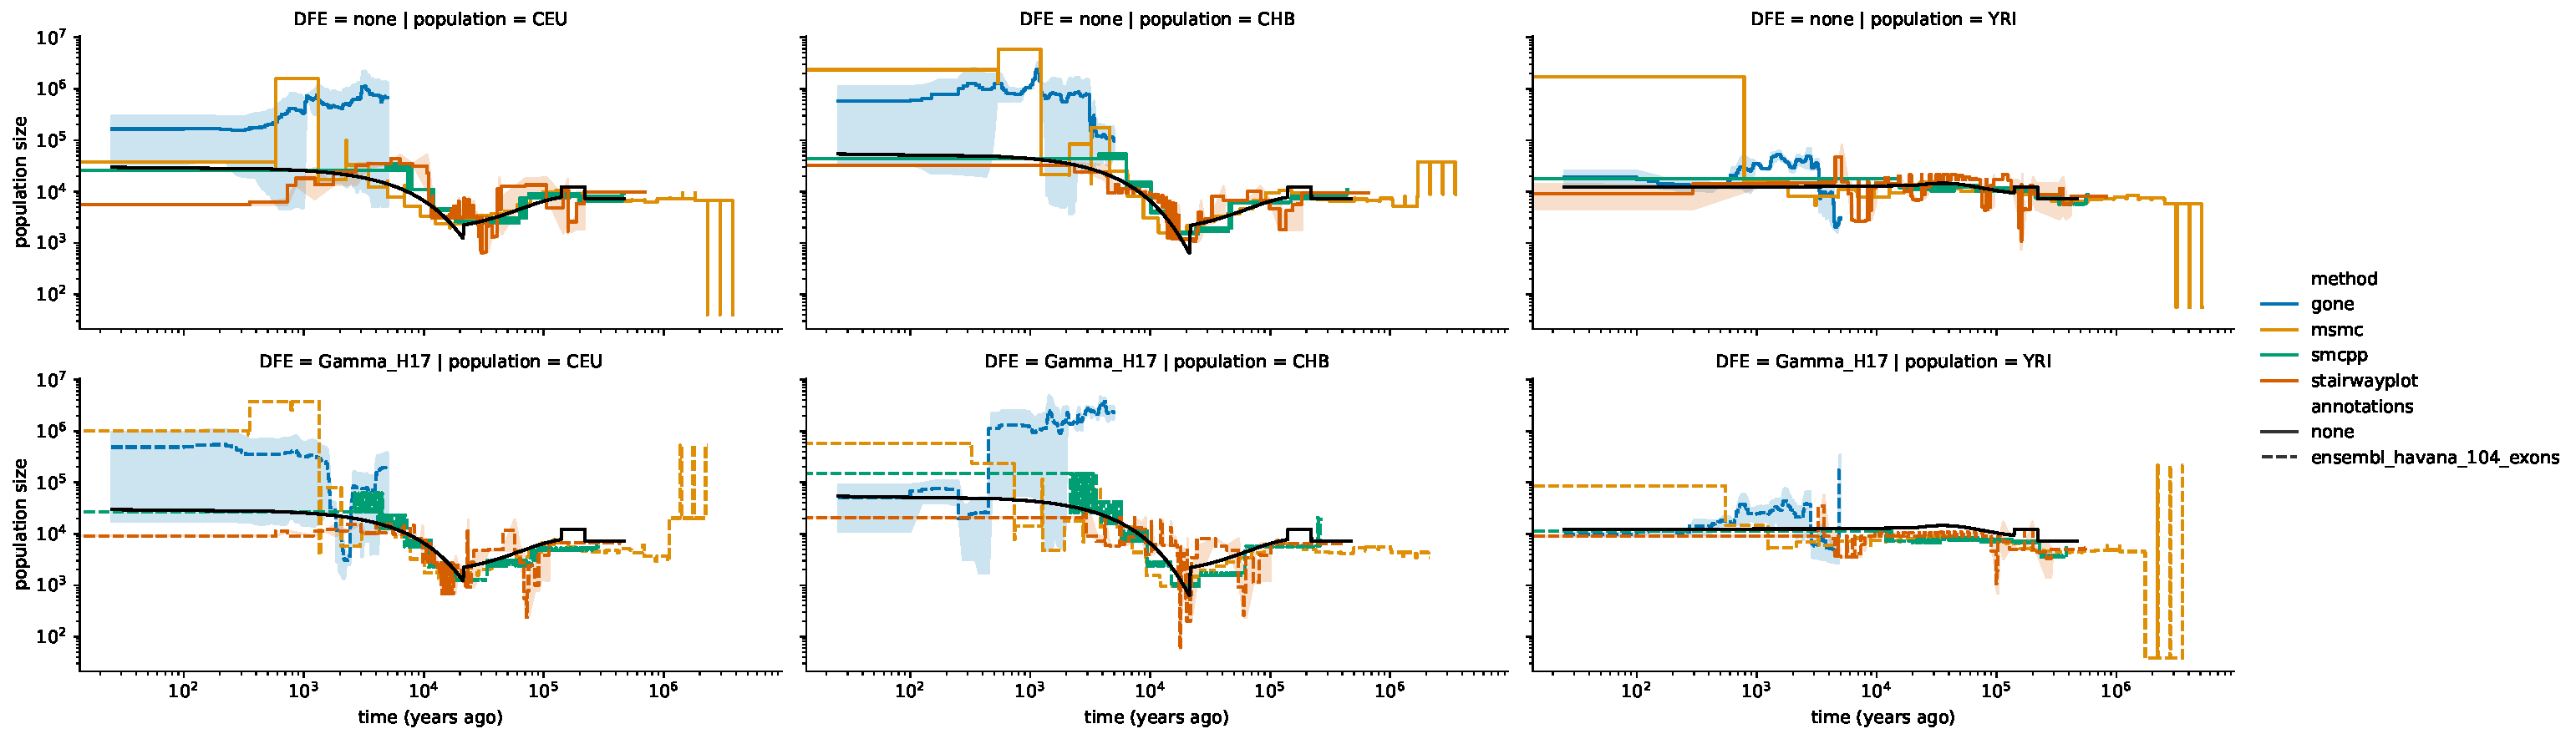
\includegraphics[width=\textwidth]{figures/HomSap/estimated_Ne_t_final}
        \caption{
        \label{fig:demography}
        Performance of methods to infer human OOA model
        with and without background selection on exons.
        }
    \end{figure}


    \begin{figure}[ht]
        \centering
        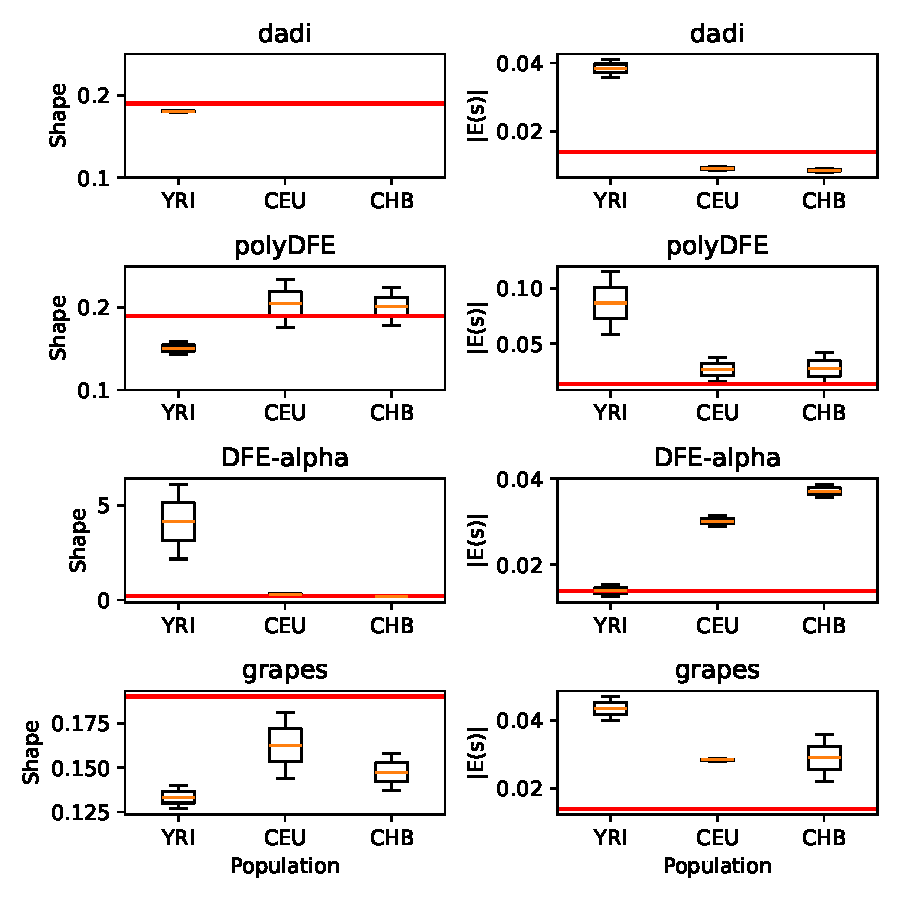
\includegraphics[width=\textwidth]{figures/HomSap/dfe.inference.benchmark}
        \caption{
        \label{fig:dfe_humans}
        Performance of methods to infer distribution of fitness effects (DFE).
        }
    \end{figure}


    \begin{figure}[ht]
        \centering
        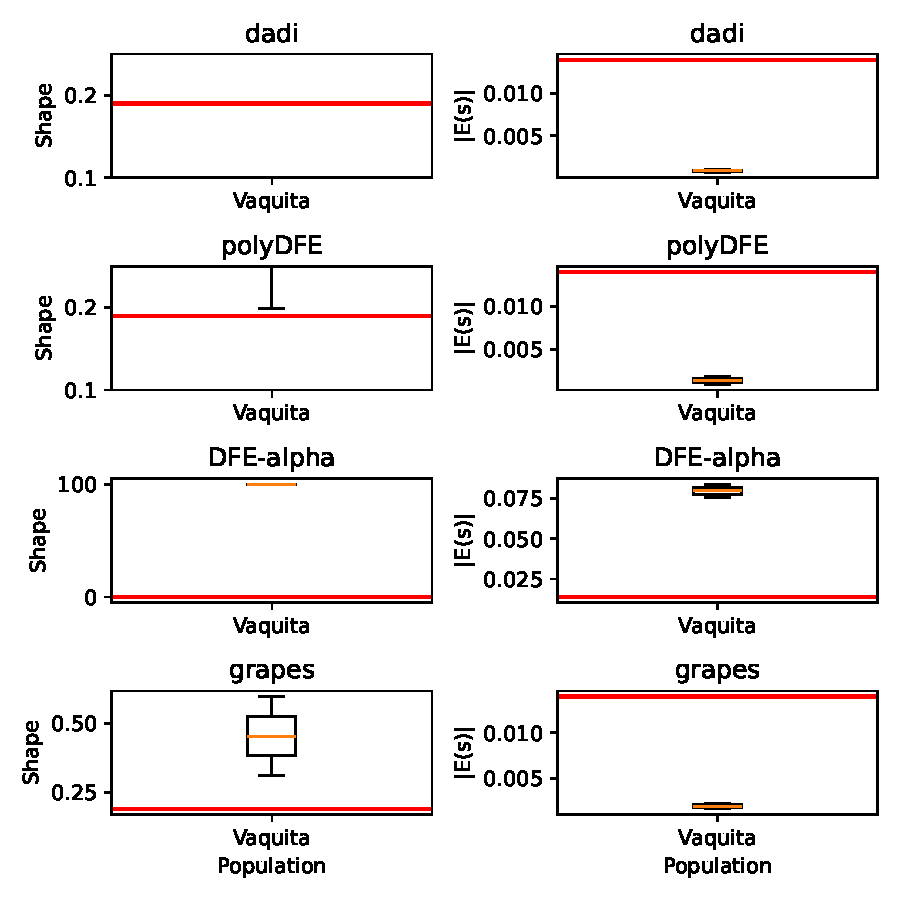
\includegraphics[width=\textwidth]{figures/PhoSin/dfe.inference.benchmark}
        \caption{
        \label{fig:dfe_vaquita}
        Performance of methods to infer distribution of fitness effects (DFE).
        }
    \end{figure}


\section*{Conclusion}
    \label{conclusion}

\section*{Data availability}\label{data_availability}


\section*{Acknowledgments}\label{acknowledgements}

\section*{Funding}
    \label{funding}

\bibliography{references.bib}
\end{document}